\documentclass[12pt]{article}

\usepackage{sbc-template}
\usepackage{graphicx,url}
\usepackage[utf8]{inputenc}
\usepackage[portuges]{babel}
     
\sloppy

\title{EASYCODE: UM AMBIENTE DE TECNOLOGIAS DE APOIO PARA O ENSINO DE LÓGICA DE PROGRAMAÇÃO}

\author{Daniela F. Feitosa \inst{1}, Eduardo N. B. Neves \inst{2}, Jucimar B. Souza \inst{1}, Emmerson S. R. Silva \inst{3} }

\address{Instituto Federal de Educação, Ciência e Tecnologia do Amazonas \\ Campus Manaus Centro (IFAM-CMC)
  \email{\{danielaferreira1133, eddunic, jucibs, emmsr2004\}@gmail.com}
}

\begin{document} 

\maketitle

\begin{abstract}
This research plan presents the scientific contribution aimed at EasyCode software, developed by IFAM-CMC students in 2017, in order to adapt it to students who have difficulty applying the programming logic of the imperative paradigm in solving computational problems. It will consist of application of the cognitive domain of the Revised Bloom Taxonomy (ANDERSON et al., 2001) together with graphical representations (flowcharts and simulators of aspects of the educational field under study), gamification based on the categories of said domain of taxonomy, and robotics in order to provide an understanding of computational problems according to the types of learning. The aim is to encourage the learning of imperative programming languages. The application of this set of methods in the teaching-learning process will allow programming concepts to be understood in a playful way.
\end{abstract}
     
\begin{resumo}
Este plano de pesquisa apresenta a contribuição científica objetivada para o software EasyCode, desenvolvido por alunos do IFAM-CMC em 2017, visando adequá-lo aos estudantes que têm dificuldade em aplicar a lógica de programação do paradigma imperativo na resolução de problemas computacionais. Consistirá na aplicação do domínio cognitivo da Taxonomia de Bloom Revisada (ANDERSON et al., 2001) em conjunto com representações gráficas (fluxogramas e simuladores de aspectos da vertente educacional em estudo), gamificação baseada nas categorias do referido domínio da taxonomia, e da robótica educacional a fim de proporcionar a compreensão de problemas computacionais de acordo com os tipos de aprendizagem. Objetiva-se incentivo ao aprendizado de linguagens da programação imperativa. A aplicação deste conjunto de métodos no processo de ensino-aprendizagem permitirá que conceitos da programação sejam compreendidos de maneira lúdica.
\end{resumo}

\section{Introdução}
As dificuldades apresentadas no ensino de programação variam desde a abordagem utilizada para o ensino, à possíveis barreiras para a acessibilidade ou aspectos psicológicos. Dentre o conjunto de fatores que inviabilizam a compreensão da programação apontados por Gomes \textit{et al}. (2008), destacam-se a falta de motivação e a complexidade das linguagens de programação utilizadas em conjunto com o 	desenvolvimento da lógica.

\section{Metodologia} 
Utilizar-se-á o domínio cognitivo da Taxonomia de Bloom Revisada para que ocorra a integração de abordagens de ensino que se adequem aos tipos de aprendizagem, considerando aspectos de adaptação dos blocos de comando.\\
A partir da implantação do recurso de feedback, a gamificação será reforçada devido à simultânea verificação da montagem dos blocos. Caso a estrutura seja correspondente aos requisitos da linguagem, ao fim da codificação o sistema exibirá uma mensagem de congratulação pela conquista de acerto do código requerido.\\
No processo de desenvolvimento deste projeto serão realizadas pesquisas com o público-alvo, especificamente alunos que possuem dificuldades em entender questões a respeito da vertente educacional a ser estudada. Por meio de perguntas a respeito da compreensão da referente lógica de programação com pessoas que possuem dificuldades ao estudá-la, será possível avaliar o nível de desenvoltura na resolução auxiliada com o software EasyCode. Tal procedimento auxiliará os ajustes da configuração do ambiente do software, bem como seus impasses até então dissimulados.


\section{Resultados e Discussão}
	\begin{figure}[h]
		\centering
		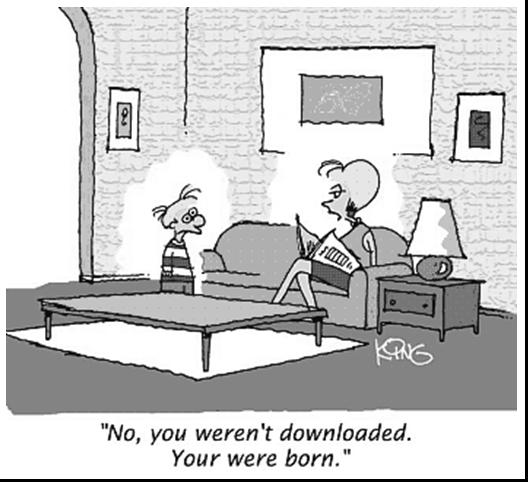
\includegraphics[scale=0.2]{fig1.jpg}
		\caption{Uma típica figura.}
		\label{fig1}
	\end{figure}

\section{Considerações Finais}
Espera-se que as mudanças propostas colaborem com o processo de ensino-aprendizagem, por exemplo, permitindo que professores possam demonstrar de forma mais lúdica conceitos da programação e também que ocorra a adequação da abordagem de ensino aos tipos de aprendizagem. 
Os consensos para a continuidade do projeto em questão possuem a intenção de aumentar a praticidade de uso do referido por meio da eficácia do planejado. 

\bibliographystyle{sbc}
\bibliography{ArtigoEC}

\end{document}